\section{Anhang}

\subsection{praktische Anwendungen der Redox Reaktionen}

\subsubsection{Inhalt} %maybe als Anhang?
\begin{itemize}
	\item galvanische Zellen
	\item  Batterien und Akkus
	\item  Brennstoffzellen
	\item  elektrolytische Verfahren
	

\end{itemize}

\subsection{Flüssigkristalle}

\subsubsection{Definition}

\subsubsection{Molekülstruktur}

\subsubsection{TN-Zelle (Twisted Nematic)}
\begin{minipage}{0.48\linewidth}
	\begin{center}
		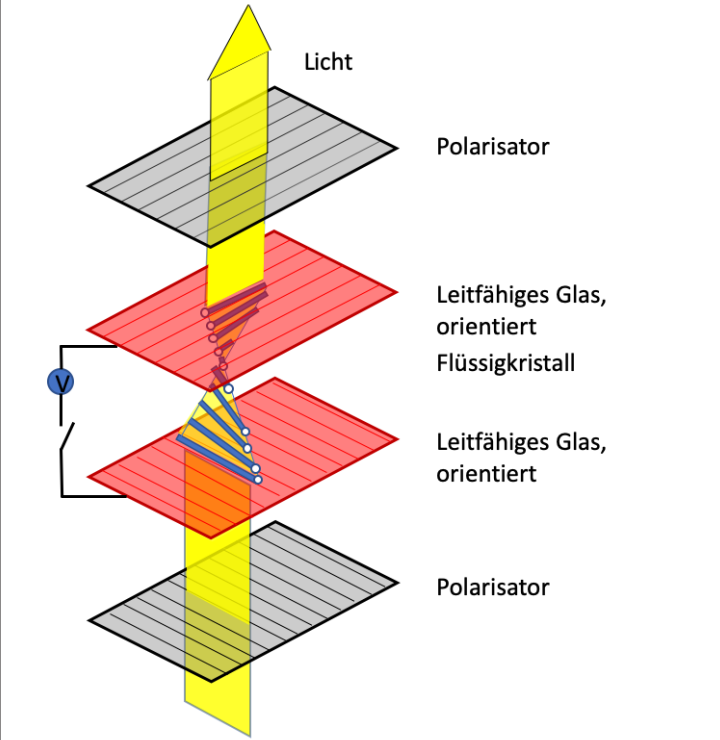
\includegraphics[width=0.8\linewidth]{images/TN-Zelle1.png}
		
		ohne angelegte Spannung   
	\end{center}
\end{minipage}
\hfill
\begin{minipage}{0.48\linewidth}
	\begin{center}
		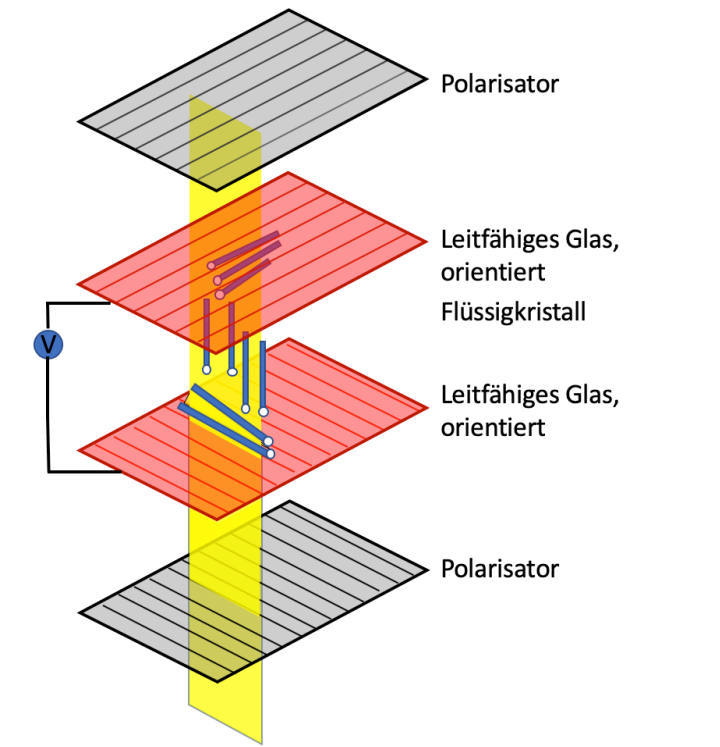
\includegraphics[width=0.8\linewidth]{images/TN-Zelle2.png} 
		
		mit angelegter Spannung 
	\end{center}
\end{minipage}



